% gepisat_appdx_b.tex
%
% written by Tyler W. Davis
% Imperial College London
%
% 2014-10-29 -- created
% 2014-10-29 -- last updated
%
% ------------
% description:
% ------------
% This TEX file contains Appendix B: Resampling MODIS for the GePiSaT model documentation.
%
% ----------
% changelog:
% ----------
% 01. modularized chapter [14.10.29]
% 02. newline for each sentence [14.10.29]
% --> simpler for Git version control
%
%% \\\\\\\\\\\\\\\\\\\\\\\\\\\\\\\\\\\\\\\\\\\\\\\\\\\\\\\\\\\\\\\\\\\\\\\\ %%
%% APPENDIX B -- RESAMPLING MODIS
%% //////////////////////////////////////////////////////////////////////// %%
\section{Resampling MODIS Data:}
\label{app:modis}
To upscale MODIS 0.05$^{\circ}$ resolution data to model-defined 0.5$^{\circ}$ resolution, there are two methods which can be employed.  
The first method is considered the long-hand method where each MODIS raster image is resampled through the Quantum GIS (QGIS) software\footnotemark.\footnotetext{\url{http://qgis.org}}  
The second method, considered the quicker automated method, utilizes Python to resample the MODIS data directly from the HDF files.

%% \\\\\\\\\\\\\\\\\\\\\\\\\\\\\\\\\\\\\\\\\\\\\\\\\\\\\\\\\\\\\\\\\\\\\\\\ %%
%% APPENDIX B.1 -- THE QGIS METHOD
%% //////////////////////////////////////////////////////////////////////// %%
\subsection{The QGIS method}
\label{app:modqgis}
The first step in processing MODIS data in QGIS is exporting the variable of interest from the HDF file to ASCII raster file format. 
This is accomplished in Python.

\begin{enumerate}
    \item Import ASCII raster file in QGIS
    \item Create 0.5$^{\circ}$ fishnet:
    \begin{enumerate}
        \item Vector $\rightarrow$ Research Tools $\rightarrow$ Vector Grid
        \item Set extents for longitude, xmin: -180.0; xmax: 179.5
        \item Set extents for latitude, ymin: -89.5; ymax: 90.0 
        \item Set grid cell size, x: 0.5; y: 0.5
        \item Save the output grid as polygons
        \item Add new fields in shapefile attribute table:
        \begin{enumerate}
            \item Output field: ``LAT''\\
                  Type: Real (width: 6; precision: 2)\\
                  Expression: \texttt{0.5 * (``YMAX'' + ``YMIN'')}
            \item Output field: ``LON''\\
                  Type: Real (width: 7; precision: 2)\\
                  Expression: \texttt{0.5 * (``XMAX'' + ``XMIN'')}
            \item Output field: ``STATION''\footnotemark\\
                  Type: Whole number (width: 8)\\
                  Expression: \texttt{720.0 * (359.0 - ((90.0 - ``LAT'')/0.5 \\
                  - 0.5)) + ((``LON'' + 180)/0.5 - 0.5)}
                  \footnotetext{The ``STATION'' field is calculated based on the 
                  conversion of the numbering index of the MODIS 0.05$^{\circ}$ 
                  to that of the WATCH WFDEI 0.5$^{\circ}$ grid. See equations 
                  \ref{eq:modisxa}--\ref{eq:modis2watch}.}
        \end{enumerate}
    \end{enumerate}
    \item Add fishnet to map
    \item Polygonize MODIS raster:
    \begin{enumerate}
        \item Vector $\rightarrow$ Conversion $\rightarrow$ Polygonize
        \item Input: MODIS raster layer
        \item Output: Polygon shapefile layer
    \end{enumerate}
    \item Intersect fishnet and polygonized MODIS layers:
    \begin{enumerate}
        \item Vector $\rightarrow$ Geoprocessing Tools $\rightarrow$ Intersect
        \item Input: Fishnet layer
        \item Intersect: Polygonized MODIS layer
        \item Output: Intersected polygon shapefile layer
    \end{enumerate}
    \item Calculate stats:
    \begin{enumerate}
        \item Load plugin: Group stats
        \item Plugins $\rightarrow$ Group Stats $\rightarrow$ Group Stats
        \item Vector: Intersected layer
        \item Classification: ``STATION'' field
        \item Value: ``DN'' field
        \item Calculate statistics and save to CSV file
    \end{enumerate}
    \item Load statistics CSV file as a table (via Vector import)
    \item Join table attributes to fishnet layer
    \begin{enumerate}
        \item Join: ``STATION'' field
        \item Target: ``STATION'' field
    \end{enumerate}
    \item Save fishnet layer as a new shapefile
    \item Create a new field in attribute table:
    \begin{enumerate}
        \item Output field: ``EVIZ''\\
              Type: Whole number (width: 5)\\
              Expression: \texttt{CASE WHEN ``Average'' IS NULL THEN -3000 \\
              ELSE toint(``Average'') END}
    \end{enumerate}
    \item Rasterize polygon layer (based on ``EVIZ'' field)
\end{enumerate}

\noindent It should be noted that the MODIS pixels are indexed starting at zero at the top left corner (north-west most pixel) and are row-major ordered ending with the last pixel in the bottom-right corner (south-east most pixel).  
On the contrary, the WATCH pixels are indexed starting at zero in the bottom-left corner (south-west most pixel) and is row-major ordered ending at the top-right corner (north-west most pixel).  
The STATION expression shown above starts by first converting the longitude (i.e., ``LON'' field) and latitude (i.e., ``LAT'' field) to equivalent MODIS 0.05$^{\circ}$ $x_{a}$ and $y_{a}$ indices:

%% ---------------------------------------------------------------%%
%% eq:modisxa | Conversion from longitude to x-index (MODIS)
%% ---------------------------------------------------------------%%
\begin{equation}
\label{eq:modisxa}
    x_{a} = \frac{\text{``LON''} + 180}{0.05} - 0.5
\end{equation}

%% ---------------------------------------------------------------%%
%% eq:modisya | Conversion from latitute to y-index (MODIS)
%% ---------------------------------------------------------------%%
\begin{equation}
\label{eq:modisya}
    y_{a} = \frac{90 - \text{``LAT''}}{0.05} - 0.5
\end{equation}

To address the different origins between the two numbering schemes, the MODIS row number, $y_{a}$, is subtracted from the largest row number to get the WATCH row index, (i.e., $y_{b} = 359 - y_{a}$).  
The column numbering is the same for both schemes (i.e., $x_{b} = x_{a}$). 
Finally the WATCH station numbering scheme is applied:

%% ---------------------------------------------------------------%%
%% eq:modis2watch | STATION equation
%% ---------------------------------------------------------------%%
\begin{equation}
\label{eq:modis2watch}
    \text{``STATION''} = 720 \cdot y_{b} + x_{b}
\end{equation}

%% \\\\\\\\\\\\\\\\\\\\\\\\\\\\\\\\\\\\\\\\\\\\\\\\\\\\\\\\\\\\\\\\\\\\\\\\ %%
%% APPENDIX B.2 -- THE PYTHON METHOD
%% //////////////////////////////////////////////////////////////////////// %%
\subsection{The Python method}
\label{app:modpy}
The Python method, instead of exporting raster images, processes the data directly from the HDF file.  
The methodology is similar to the QGIS method in that MODIS 0.05$^{\circ}$ resolution pixels are averaged to 0.5$^{\circ}$ resolution.  
To circumvent the long method presented previously, Python takes advantage of the pixel numbering scheme as explained in equations \ref{eq:modisxa}--\ref{eq:modis2watch}.  
The Python procedure begins by iterating through each of the 0.5$^{\circ}$ pixels (i.e., 360 $\times$ 720 pixel grid).  
For each 0.5$^{\circ}$ pixel, the 100 0.05$^{\circ}$ pixels are identified that exist within it.  
This is accomplished by iterating over the boundary box calculated based on the centroid coordinates of the 0.5$^{\circ}$ pixel.  
Each of the 100 0.05$^{\circ}$ pixels are iterated over and valid EVI values are saved to an array.  
The valid EVI values in the array are averaged and the average EVI is assigned to the 0.5$^{\circ}$ pixel.  
This is repeated for all 0.5$^{\circ}$ pixels. 

%% ------------------------------------------------------------------------ %%
%% fig:gapfill | Linear model parameter estimates : optimized
%% ------------------------------------------------------------------------ %%
\begin{figure}[b!]
    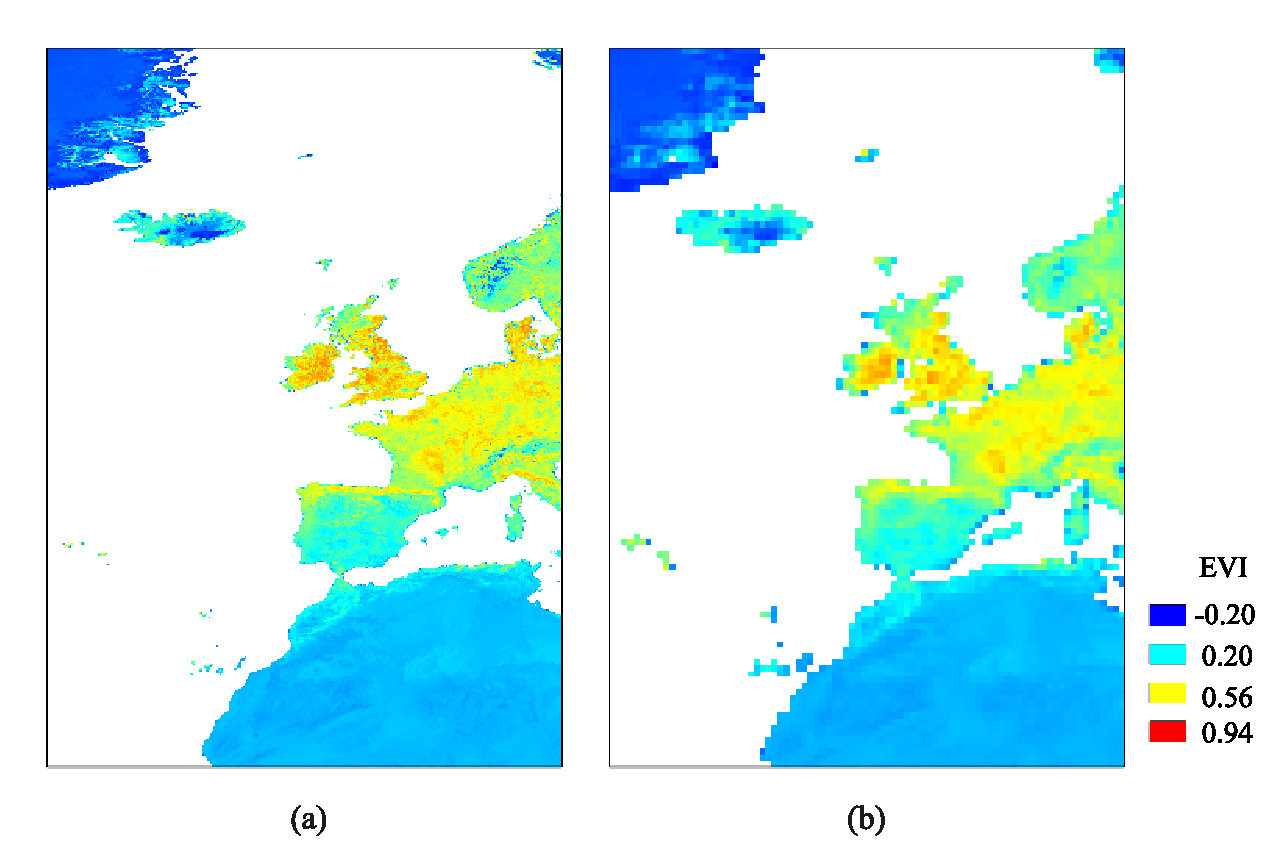
\includegraphics[width=\textwidth]{re_modis.eps}
    \caption{Pseudo-colored raster images of monthly EVI over western Europe, 
    (i.e., longitude: -30$^{\circ}$--13$^{\circ}$, latitude: 
    80$^{\circ}$--20$^{\circ}$), for June 2002 at (a) 0.05$^{\circ}$ resolution 
    and (b) 0.5$^{\circ}$ resolution (via the Python method).}
    \label{fig:remodis}
\end{figure}

Figure \ref{fig:remodis} shows two raster images of MODIS EVI at the original 0.05$^{\circ}$ resolution (Figure \ref{fig:remodis}a) and at the upscaled 0.5$^{\circ}$ resolution by the Python method (Figure \ref{fig:remodis}b).  
While the upscaling removes the finer detail from the image, the general trends in spatial EVI are well maintained. 
The re-sampling also reduces the amount of data storage required by a factor of $\approx$100 (e.g., 148 MB $\rightarrow$ 1.5 MB).  
